\documentclass{standalone}
\usepackage{graphicx}	
\usepackage{amssymb, amsmath, amsthm}
\usepackage{color}

\usepackage{tikz}
\usetikzlibrary{math}

\definecolor{light}{RGB}{220, 188, 188}
\definecolor{mid}{RGB}{185, 124, 124}
\definecolor{dark}{RGB}{143, 39, 39}
\definecolor{highlight}{RGB}{180, 31, 180}
\definecolor{lightteal}{RGB}{107, 142, 142}
\definecolor{midteal}{RGB}{72, 117, 117}
\definecolor{darkteal}{RGB}{29, 79, 79}
\definecolor{gray10}{gray}{0.1}
\definecolor{gray20}{gray}{0.2}
\definecolor{gray30}{gray}{0.3}
\definecolor{gray40}{gray}{0.4}
\definecolor{gray60}{gray}{0.6}
\definecolor{gray70}{gray}{0.7}
\definecolor{gray80}{gray}{0.8}
\definecolor{gray90}{gray}{0.9}
\definecolor{gray95}{gray}{0.95}

\begin{document}

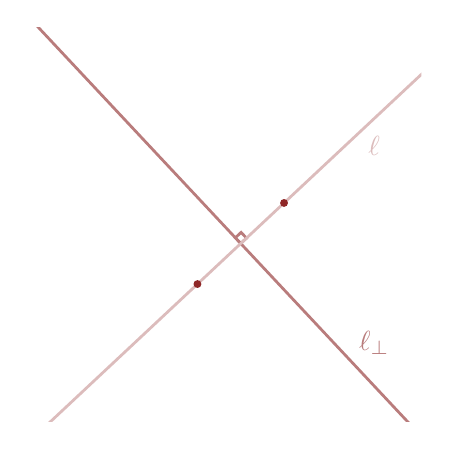
\begin{tikzpicture}[scale=2]
  \clip (-0.75, -0.75) rectangle (1.75, 1.75);
  
  \fill[white] (-2, -2) rectangle (2, 2);
  
  \pgfmathsetmacro{\xa}{0.878}
  \pgfmathsetmacro{\ya}{0.637}

  \pgfmathsetmacro{\xb}{0.328}
  \pgfmathsetmacro{\yb}{0.122}
  
  \pgfmathsetmacro{\xab}{(\xa + \xb) / 2}
  \pgfmathsetmacro{\yab}{(\ya + \yb) / 2}
  
  \pgfmathsetmacro{\mab}{ ( \yb - \ya ) / ( \xb - \xa ) }
  \pgfmathsetmacro{\mabp}{-1 / \mab}

  \pgfmathsetmacro{\delta}{0.05}
  \draw[mid, line width=1, rotate around={atan(\mab):(\xab, \yab)}] 
    ( \xab, \yab ) rectangle +(\delta, \delta);
  
  \draw[mid, line width=1] 
     ( -4, { \mabp * (-4 - \xab ) + \yab }) -- ( 4, { \mabp * (4 - \xab ) + \yab });
  \draw[light, line width=1] 
    ( -4, { \mab * (-4 - \xab ) + \yab }) -- ( 4, { \mab * (4 - \xab ) + \yab });
  
  \foreach \x/\y in { 0.878/0.637, 0.328/0.122 } {
    \fill[dark] (\x, \y) circle (0.025);
  }
  
  \node[light] at (1.45, 1) { $\ell$ };
  \node[mid] at (1.45, -0.25) { $\ell_{\perp}$ };
  
\end{tikzpicture}

\end{document}  